\section{Baseline Architecture}

    \begin{figure}
        \begin{center}
            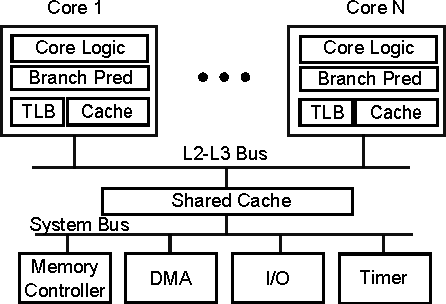
\includegraphics[width=3in]{figs/baseline.pdf}
            \caption{The timing-channel vulnerable baseline architecture.}
            \label{fig:baseline}
        \end{center}
    \end{figure}

    Figure \ref{fig:baseline} shows the baseline architecture which is later 
    extended to include timing channel protection. The architecture has 
    multiple cores, each with a branch predictor, one or more private caches, a 
    TLB, and the core logic. Each processor is connected to a shared cache 
    through an on-chip network. The multicore processor is connected to the 
    main memory and a DMA module through the system bus. 

    The hardware is concurrently shared by multiple security domains. A 
    security domain consists of one or more software modules (such as processes 
    or threads in a single OS system or virtual machines in a virtualization 
    based system). Software modules within the same security domain trust each 
    other, but information flows between security domains must be controlled 
    according to a policy that meets the security requirements of the system.
    Often, this policy entails of a lattice of security levels such as 
    $\mathtt{normal} \sqsubseteq \mathtt{secure}$, where the information 
    available to a security domain includes any information available to 
    security domains at its own level and all levels that preceed it in the 
    lattice order.  In another model, security domains can be mutually 
    distrusting and no information can be shared between them. (This cannot be 
    expressed as a lattice, since even if you have domains which are all 
    incomparable, each pair of elements does not have a supremum and infimum).  
    As shown in Figure \ref{fig:baseline}, it is possible for a security domain 
    to have multiple virtual machines which may be allocated to different 
    cores. It is also possible for security domains to be time multiplexd on 
    the same core (e.g.  by context switching VMs), but it is not possible for 
    security domains to execute concurrently on the same core (e.g. through 
    SMT).

\section{Usage Scenarios and Threat Models}

    This section describes some example applications for the architecture and 
    the thread model for each usage scenario.

    \subsection{DRM Video Playback}
    Mobile devices often support applications that playback videos with
    DRM restrictions. For example, a user may only be able to play a video if 
    he or she has a valid subscription to the service. In this case, the 
    attacker is the owner of the mobile device who would either like to access 
    content without paying for a subscription. The adversary is capable of any 
    software attack in addition to simple physical attacks, for example, by 
    making power measurements at the terminals of the SoC to carry out a 
    differential power analysis attack. However, power side channel attacks are 
    orthogonal to the problems addressed in this work and viable solutions 
    already exist \cite{needed}. Since all software attacks are possible, the 
    adversary is capable of performing timing channel attacks. 

    \subsubsection{DRM Protection Security Mechanisms}
    AMD TrustZone \cite{trustzone} exemplifies a state of the practice solution 
    that can enforce these security properties, however, TrustZone does not 
    offer protection against timing channel attacks. Since the adversary can 
    carry out any software attack and timing channels can be exploited with 
    software attacks, timing channel protection is necessary to meet the 
    security requirements. 

    \begin{figure}
        \begin{center}
            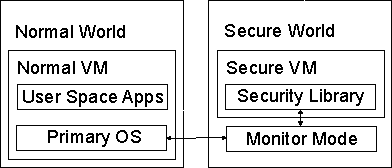
\includegraphics[width=3in]{figs/worlds.pdf}
            \caption{The security domains of TrustZone-like processor.}
            \label{fig:tz_domains}
        \end{center}
    \end{figure}
    
    TrustZone separates the software modules into two security domains as shown 
    in Figure \ref{fig:tz_domains} . The first security domain is called the 
    normal world and it has a virtual machine that contains the operating 
    system and all user-space applications. The other security domain, the 
    secure world, contains a virtual machine that contains only a small 
    execution environment and a set of very simple libraries for handling 
    protected operations. This VM does not contain a complete operating system 
    and the libraries do not require any operating system support (e.g. they 
    may not have system calls). The secure world also contains software for a 
    simple monitor mode that handles context switching between the two domains 
    if they are time multiplexed on the same core. The security levels of these 
    domains form a lattice such that the level of the normal world precedes the 
    level of the secure world (i.e. information available to the normal world 
    is available to the secure world). All of the secure world code is small to 
    reduce the chance of vulnerabilities. The secure world must only allow the 
    normal world to play the video if the subscription is valid. 


    \begin{figure}
        \begin{center}
            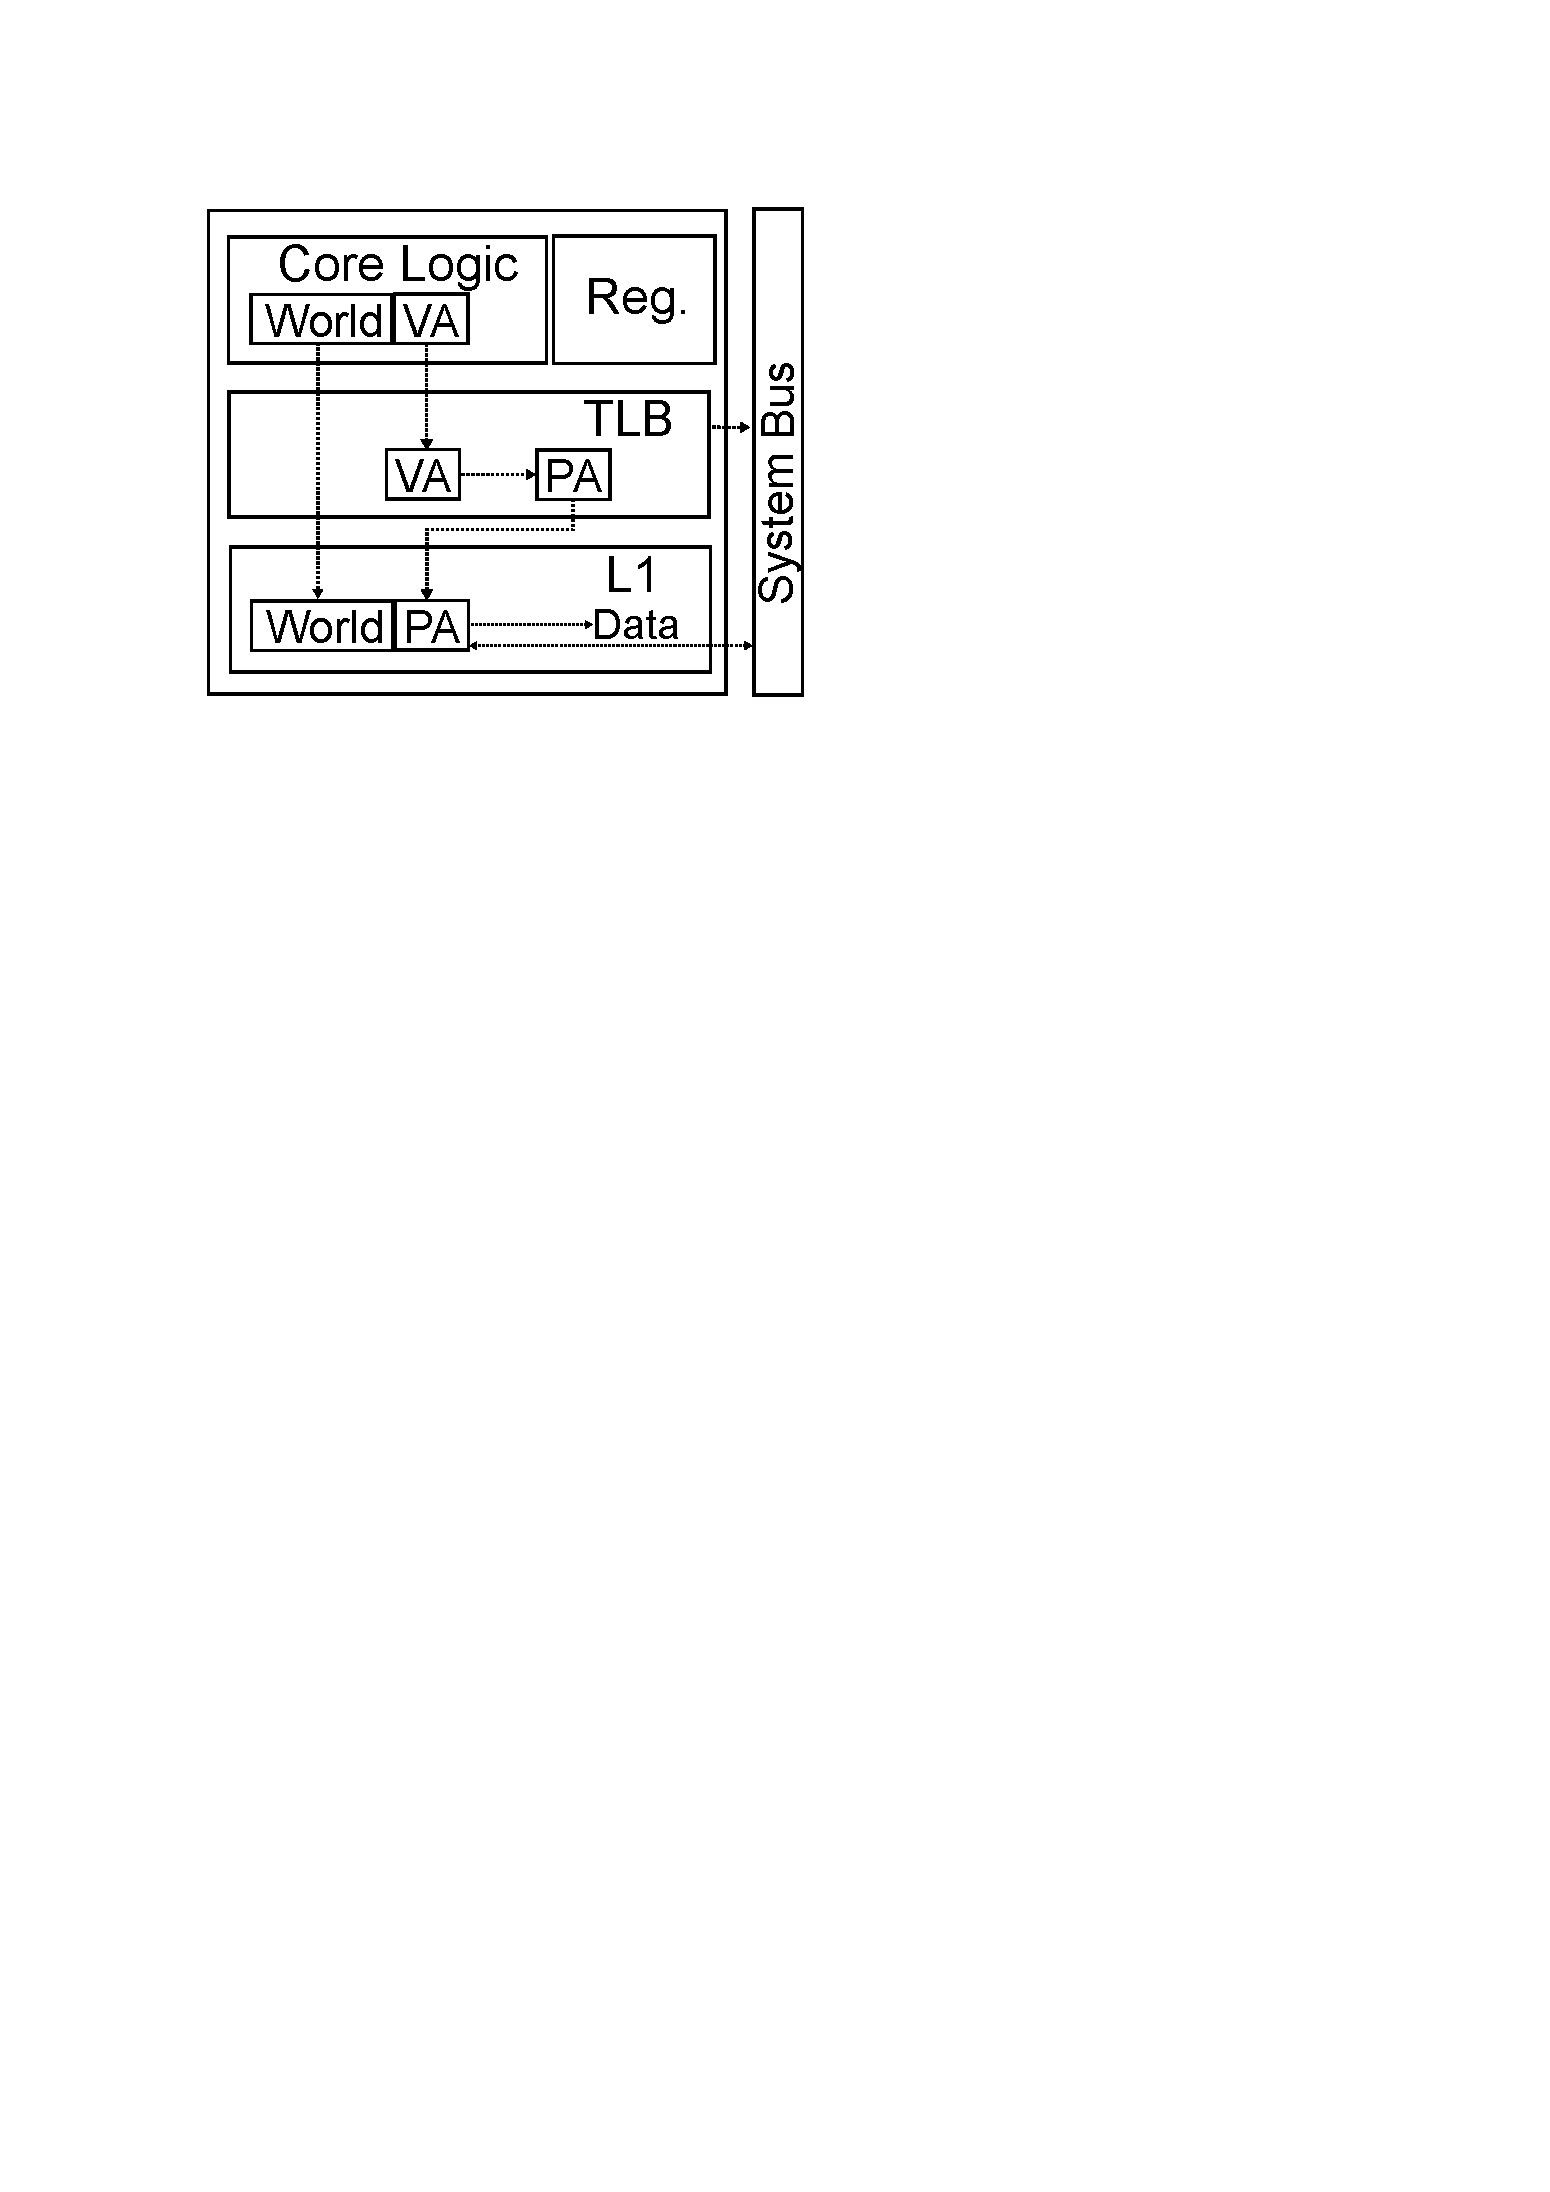
\includegraphics[width=3in]{figs/tz_tags.pdf}
            \caption{DRM Protection Mechnamisms. The baseline architecture is 
            extended with tags that control explicit information flows between 
        the secure and normal worlds.}
            \label{fig:baseline}
        \end{center}
    \end{figure}

    TrustZone extends the baseline cores of Figure \ref{fig:baseline} to
    those shown in Figure \ref{fig:tz_uarch}. The core logic contains a tag to 
    store which world is currently executing. Each cache entry has a tag to 
    indicate if the entry can be accessed by the normal world or not. To make 
    an access to the memory hierarchy, the core sends the virtual address and 
    the current world to the TLB. The TLB gets the physical address as normal 
    (performing a page table walk if needed). The physical address and current 
    security domain are sent to the cache. If the cache contains the physical 
    address and the tag of the entry indicates that the current world has 
    sufficient rights to accesss the entry, the access proceeds normally.  
    Otherwise, if it is a cache miss, the cache sends the physical address and 
    the current world to the system bus to access the main memory. If the tag 
    of the address in main memory indicates that the current world has 
    sufficient rights, the cache block is brought into the cache as normal and 
    the tag is set in the cache. If it is either a hit or a miss and the 
    security level does not meet the requirements, the access fails.

    The two virtual machines may share the same physical processor in 
    time-multiplexed way through context switching. Context switches between 
    these VMs are entered by a special instruction that invokes the monitor 
    mode.  Typically, the monitor mode will save the general purpose registers 
    and any processor configuration registers. The TLB and caches are not 
    flushed since the tags protect illegal data accesses.

    To play the DRM protected video, it is sent to the device through an 
    encrypted stream. The key used for decryption is stored inside the secure 
    world VM. To play the video, the user space application loads the encrypted 
    data into the cache, tagging it as normal world readable. It then issue a 
    special instruction to interact with the secure world which decrypts the 
    stream. This invokes the monitor mode which then context switches out the 
    normal world VM replacing it with the secure world VM. The secure world VM 
    loads the encrypted data into the cache, decrypts it with a key that is 
    only readable by the secure world, tags it as readable by the normal world, 
    and invokes the monitor to return execution to the normal world. Note that 
    the data is not cleared from the TLB or cache during context switches.  The 
    normal world and secure world VMs can execute in separate cores which 
    communicate through the shared cache instead of context switching, however, 
    since they operate on the same data, it is generally better if they share 
    the same core allowing them to both access the data quickly in the private 
    cache.
